\section{System Design \& Failure Modes}
\label{sec:design}

We contend that normative authorization, the question of who ought to receive
a document, is outside the scope of what an LLM can be trusted to decide. The \textit{Privacy Conductor} architecture therefore evaluates each information flow with a \textit{deterministic} gate and permits or denies it before the LLM sees the data. Throughout this study, we assume all participants act in good faith; our concern is inadvertent disclosure.

\subsection{System Roles and Protected Assets}
Our architecture consists of five participants. The \emph{Requester}, whose role is determined by context, interacts with the LLM-based \emph{Assistant}. The \emph{Assistant} accesses the labeled-document \emph{Store} only through the \emph{Conductor}, which permits or denies requests according to policies defined by the \emph{Policy Authority}. The authority may be an individual, organization, legislation such as HIPAA, or another authoritative policy source. This mediation keeps the LLM-based \emph{Assistant} outside the trust boundary, as shown in Fig.~\ref{fig:architecture}.

An LLM may occupy two roles in this design. As the \emph{Assistant}, it is untrusted. As a \emph{labeler}, it may generate policy-relevant labels and therefore assumes a trusted role. Section~\ref{sec:substitution} evaluates whether an LLM can reliably serve in this capacity.

The system protects three assets: documents, their labels, and the assignment relations linking requesters to subjects or roles. Because the \emph{Conductor} relies on the latter two for access decisions, corrupted labels or relations can cause incorrect policy enforcement.

%Our architecture contains five participants. The {\em Requester}, an actor with a contextually determined role, interacts with the {\em Assistant}, an LLM. The {\em Assistant} reaches the {\em Store}, a collection of labeled documents, only through the {\em Conductor}, which permits or denies each access using policy written by the {\em Policy Authority}: an individual, a group, legislation (e.g., HIPAA), or any other source of policy. This moves the LLM out of the trust boundary (as shown in Fig.~\ref{fig:architecture}).

%An LLM could occupy two positions in this design. As the {\em Assistant}, it is untrusted. As a \emph{labeler}, it would act as the {\em Policy Authority}, which is fully trusted. Section~\ref{sec:substitution} further tests and evaluates whether a model can fill the second role.

%Three things are protected: the documents, their labels, and the assignment relation recording which requesters hold which subjects. A corrupted label or
relation makes the gate enforce the wrong policy.

\begin{figure}[!t]
  \centering
  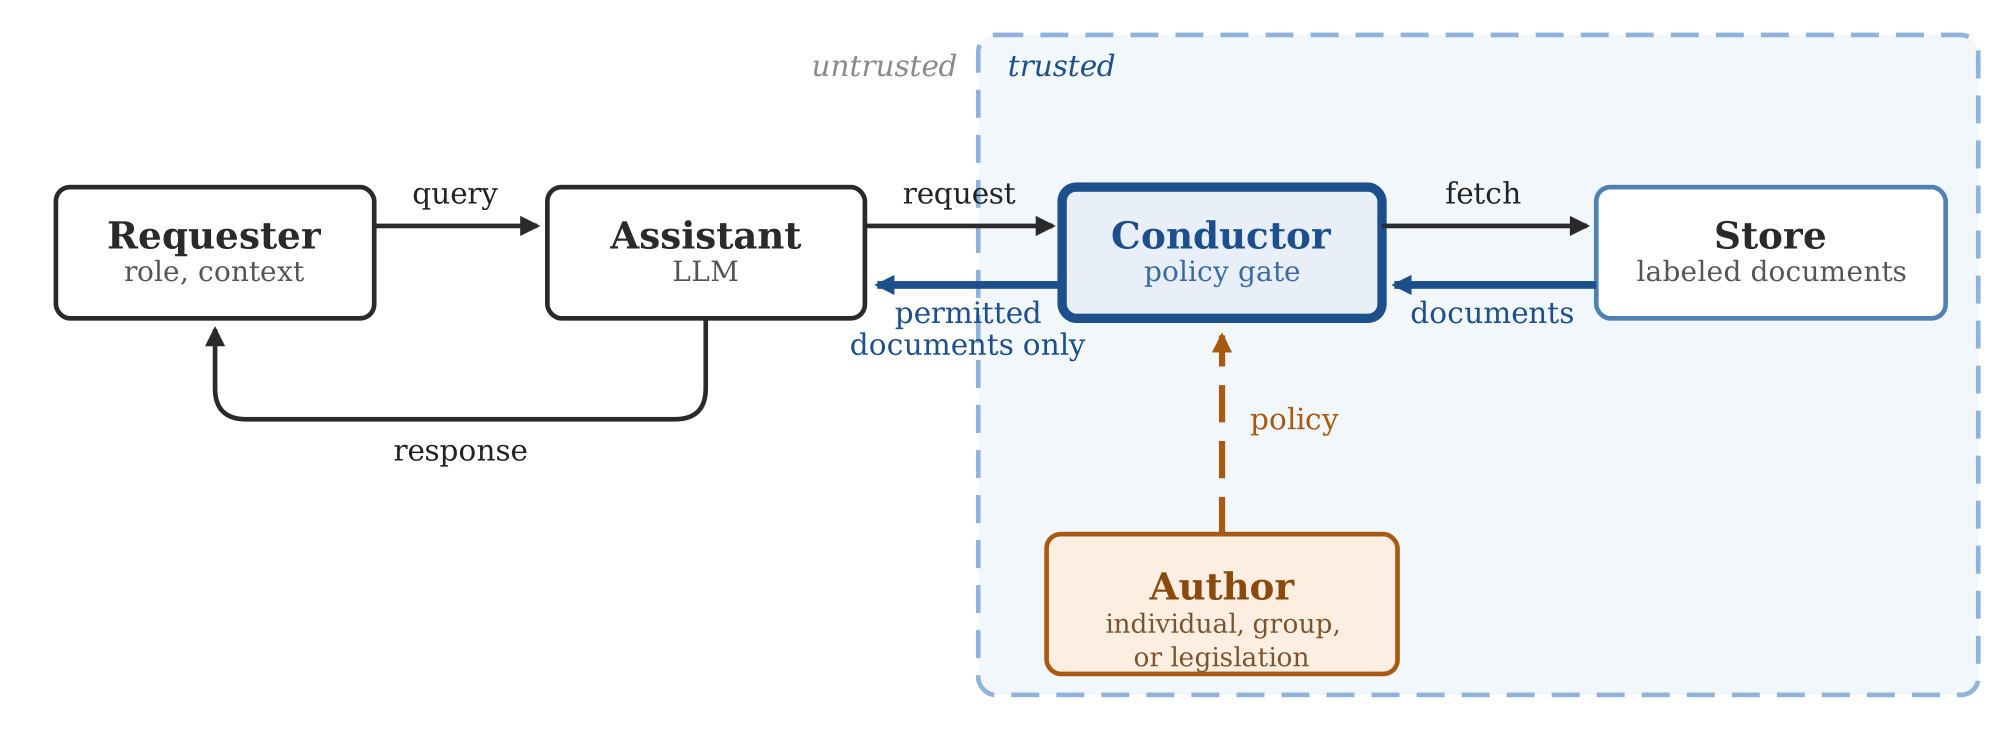
\includegraphics[width=\columnwidth]{figures/conductor-architecture.png}
  \caption{The Privacy Conductor architecture. The Assistant reaches the Store
  only through the Conductor, which applies a policy supplied out of band by
  the Policy Authority. Because the Assistant sits outside the trust boundary,
  it cannot disclose a record it was never given.}
  \label{fig:architecture}
\end{figure}

\subsection{Design Principles}
The proposed architecture rests on six design principles: %each of which is implemented or evaluated in the paper.

\begin{enumerate}
  \item \textbf{Determinism at the enforcement point.} Identical policy, label,
  and Requester yield an identical decision on every evaluation.
  \item \textbf{Default deny.} A flow that cannot be affirmatively permitted is
  refused.
  \item \textbf{No privilege amplification.} The Assistant inherits the
  Requester's permissions exactly; it holds no credentials of its own.
  \item \textbf{Authoritative policy provenance.} Every policy originates from
  an accountable Policy Authority and is thereafter applied mechanically.
  \item \textbf{Separation of labeling from enforcement.} Because the gate is
  faithful to the label it receives, a failure is localized to a single rule
  or label and is repairable by editing it.
  \item \textbf{Request text is not an input to the access decision.} The
  Conductor uses the Requester's role and the document's label, so no phrasing
  of a query can widen what is delivered.
\end{enumerate}

\subsection{The Retrieval Path}
\label{sec:retrievalpath}
Placing a decision point between an {\em Assistant} and a {\em Store} leaves
open when in the retrieval sequence the decision is taken: if candidates are
ranked over sensitive content before authorization runs, the ordering itself
can carry information the {\em Requester} is not entitled to. We therefore
specify the sequence as query, candidate resolution, policy decision,
authorized fetch, and admission to the Assistant's context. This ordering is
possible because the {\em Conductor} reads only labels and relations, so the
gate can be evaluated over candidate identifiers before any content is fetched
(Table~\ref{tab:observability}). Our evaluation exercises the policy decision
point directly, enumerating every (Requester, document) pair.
\begin{table}[!t]
\centering
\caption{The Conductor reads labels and relations but never document content.}
\label{tab:observability}
\resizebox{0.99\linewidth}{!}{%
\begin{tabular}{llllll}
\toprule
\textbf{Component} & \textbf{Content} & \textbf{Embeddings} & \textbf{Labels} &
\textbf{Requester identity} & \textbf{Assignment} \\
\midrule
Requester           & authorized only & no  & no  & yes (self) & no  \\
Assistant (LLM)     & authorized only & no  & no  & yes        & no  \\
Candidate resolver  & identifiers only & yes & no  & no         & no  \\
Conductor (gate)    & \textbf{no}     & no  & yes & yes        & yes \\
Store               & yes             & yes & yes & no         & no  \\
\bottomrule
\end{tabular}}
\end{table}

\subsection{Failure Modes}
\label{sec:failuremodes}
Permitting a flow that should be denied and denying a flow that should be
permitted are both norm violations under Contextual
Integrity~\cite{nissenbaum}. We call these \textit{privacy violations} and
\textit{over-blocks} respectively; Section~\ref{sec:measures} specifies how
each is quantified.

The Conductor is designed to eliminate two failures. \textit{Over-retrieval}
occurs when the Assistant fetches what is relevant to a query rather than what
the Requester is permitted to see. \textit{Scope mismatch} occurs when a
Requester acting in good faith, in a legitimate workflow, reaches data outside
their role. Both are eliminated by construction: the Assistant cannot disclose
a record the Conductor never delivered.

Two further failures are upstream of the Conductor. \textit{Mislabeling} occurs
when a label does not describe its document, so the gate faithfully enforces
the wrong rule. \textit{Label instability} occurs when the same document yields
different labels on different occasions. If labels are produced once, the
deployed policy is an arbitrary draw; if they are produced at request time, as
when a model sits inside the decision, access to the same record varies from
request to request. These are the failures our evaluation measures.

Regurgitation of earlier context and hallucination are out of scope: the
{\em Conductor} governs delivery, not utterance.

\subsection{Study Assumptions}
We assume that each Requester's role and context are authenticated upstream.
The {\em Policy Authority} is trusted and authoritative by construction: the
system enforces the policy it is given, so correctness is defined relative to
that policy rather than to any external standard. This follows from how CI is
formalized, with the norm as an input. Whether a given
policy is a good one is a separate question.
